\documentclass{standalone}
\usepackage[utf8]{inputenc}
\usepackage{tikz}
\usepackage{graphicx,bm,amssymb,amsmath,amsthm}
\usetikzlibrary{positioning}

\begin{document}
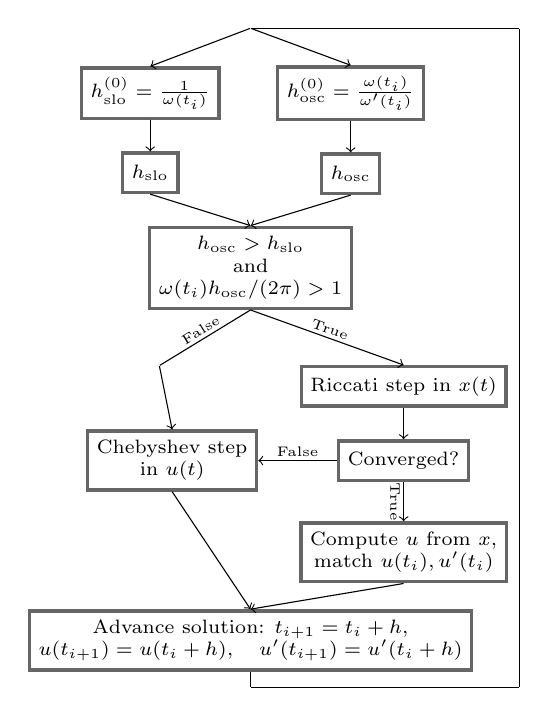
\begin{tikzpicture}[
    roundnode/.style={circle, draw=black!60, fill=green!0, very thick, minimum size=7mm},
    squarednode/.style={rectangle, draw=black!60, fill=red!0, very thick, minimum size=5mm},
    ]
    \tikzstyle{every node}=[font=\scriptsize]
    %Nodes
    \node[squarednode]      (hsloini)   {$h_{\text{slo}}^{(0)} = \frac{1}{\omega(t_i)}$};
    \node[squarednode]      (hoscini)  [right=0.7cm of hsloini] {$h_{\text{osc}}^{(0)} = \frac{\omega(t_i)}{\omega'(t_i)}$};
    \node[squarednode]      (hslo)  [below=0.4cm of hsloini] {$h_{\text{slo}}$};   
    \node[squarednode]      (hosc)  [below=0.4cm of hoscini] {$h_{\text{osc}}$};    
    \node[squarednode, align=center]      (switch) [below right=0.4cm and -0.4cm of hslo] {$h_{\text{osc}} > h_{\text{slo}}$ \\ and \\$\omega(t_i) h_{\text{osc}}/(2\pi) > 1$};
    \node[squarednode]      (ricc)  [below right=3.1cm and -1.6cm of hoscini] {Riccati step in $x(t)$};  
    \node[squarednode]      (conv)  [below=0.4cm of ricc] {Converged?}; 
    \node[squarednode, align=center]      (cheb)  [left=1cm of conv] {Chebyshev step \\ in $u(t)$}; 
    \node[squarednode, align=center]      (ic)  [below=0.5cm of conv] {Compute $u$ from $x$, \\ match $u(t_i), u'(t_i)$};     
    \node[squarednode, align=center]      (accept)  [below =3.8cm of switch] {Advance solution: $t_{i+1} = t_{i}+h$, \\ $u(t_{i+1}) = u(t_i + h), \quad u'(t_{i+1}) = u'(t_i + h)$ };    
    \node[inner sep=0, minimum size=0, below left=0.7cm and -0.15cm of switch] (k) {}; % invisible node
    \node[inner sep=0, minimum size=0, below=0.2cm  of accept] (l) {}; % invisible node
    \node[inner sep=0, minimum size=0, right=3.4cm of l] (m) {}; % invisible node
    \node[inner sep=0, minimum size=0, above=2.5cm of switch] (o) {}; % invisible node
    \node[inner sep=0, minimum size=0, right=3.4cm of o] (n) {}; % invisible node   
    
    %Lines
    \draw[->] (hsloini.south) -- (hslo.north);
    \draw[->] (hoscini.south) -- (hosc.north);
    \draw[->] (hosc.south) -- (switch.north);
    \draw[->] (hslo.south) -- (switch.north);
    \draw[->] (switch.south) -- (ricc.north) node[midway, above=-0.5ex, sloped] {\tiny True};    
    \draw[-] (switch.south) -- (k) node[midway, above=-0.5ex, sloped] {\tiny False};  
    \draw[->] (k) -- (cheb.north) ;
    \draw[->] (conv.south) -- (ic.north) node[midway, below=-0.5ex, sloped] {\tiny True};    
    \draw[->] (conv.west) -- (cheb.east) node[midway, above=-0.5ex] {\tiny False};
    \draw[->] (ic.south) -- (accept.north); 
    \draw[->] (cheb.south) -- (accept.north);    
    \draw[->] (ricc.south) -- (conv.north);
    \draw[-] (accept.south) -- (l) ;
    \draw[-] (l) -- (m) ;    
    \draw[-] (m) -- (n) ;    
    \draw[-] (n) -- (o) ; 
    \draw[->] (o) -- (hsloini.north) ;
    \draw[->] (o) -- (hoscini.north) ;    
    
\end{tikzpicture}  
\end{document}
